\documentclass[letterpaper,11pt]{article}
\oddsidemargin -1.0cm \textwidth 17.5cm

\usepackage[utf8]{inputenc}
\usepackage[activeacute,spanish, es-lcroman]{babel}
\decimalpoint
\usepackage{amsfonts,setspace}
\usepackage{amsmath}
\usepackage{amssymb, amsmath, amsthm}
\usepackage{comment}
\usepackage{float}
\usepackage{amssymb}
\usepackage{dsfont}
\usepackage{anysize}
\usepackage{multicol}
\usepackage{enumerate}
\usepackage{graphicx}
\usepackage[left=1.5cm,top=2cm,right=1.5cm, bottom=1.7cm]{geometry}
\setlength\headheight{1.5em} 
\usepackage{fancyhdr}
\usepackage{multicol}
\usepackage{hyperref}
\usepackage{wrapfig}
\usepackage{subcaption}
\usepackage{siunitx}
\usepackage{cancel}
\usepackage{mdwlist}
\usepackage{svg}
\pagestyle{fancy}
\fancyhf{}
\renewcommand{\labelenumi}{\normalsize\bfseries P\arabic{enumi}.}
\renewcommand{\labelenumii}{\normalsize\bfseries (\alph{enumii})}
\renewcommand{\labelenumiii}{\normalsize\bfseries \roman{enumiii})}


\begin{document}

\fancyhead[L]{\itshape{Facultad de Ciencias F\'isicas y Matem\'aticas}}
\fancyhead[R]{\itshape{Universidad de Chile}}

\begin{minipage}{11.5cm}
    \begin{flushleft}
        \hspace*{-0.6cm}\textbf{FI1000-1 Introducción a la Física Clásica}\\
        \hspace*{-0.6cm}\textbf{Profesora:} Jocelyn Dunstan\\
        \hspace*{-0.6cm}\textbf{Auxiliar:} Alejandro Silva\\
        \hspace*{-0.6cm}\textbf{Ayudantes:} Macarena Muñoz \& Catalina Vargas\\
    \end{flushleft}
\end{minipage}

\begin{picture}(2,3)
    \svgpath{../}  % descomentar si se agrega a carpeta "auxiliares"/"ejercicios"
    \put(366, 10){\includesvg[scale=0.31]{img/dfi.svg}}
\end{picture}

\begin{center}
	\LARGE\textbf{Auxiliar \#8:}\\
	\Large{Dinámica + Energía}
\end{center}

\vspace{-1cm}
\begin{enumerate}\setlength{\itemsep}{0.4cm}

\rfoot[]{pág. \thepage}

\item[]

\item Un cubo de masa $M$, que posee un hueco esférico de radio $R$, descansa en un orificio de superficies rectas y sin roce. Al interior del cubo hay una bolita de masa $m$ que gira sin ayuda externa en un trayecto circunferencial que pasa por el punto más bajo del hueco. En tal punto la bolita tiene rapidez $v_0$.

    \begin{enumerate}
        \item Determine la fuerza de contacto bolita-superficie en función del ángulo $\theta$ medido con respecto la vertical
        
        \item Determine el rango $v_0$ que garantice que la bolita nunca pierda contacto con la superficie, ni el cubo pierda contacto con el fondo del orificio.
    \end{enumerate}
    
\begin{figure}[H]
    \centering
    \svgpath{../img/aux4}
    \includesvg[width=0.35\linewidth]{cubo.svg}
\end{figure}

\item Una masa $m$ resbala, sin roce y debido a la gravedad, por la superficie de una semiesfera de radio $R$. La masa parte desde la cúspide sin velocidad inicial. Sea $P$ el punto en el cual la masa se separa de la semiesfera. Encuentre el ángulo de elevación $\theta_0$ del punto P.

\begin{figure}[h!]
    \centering
    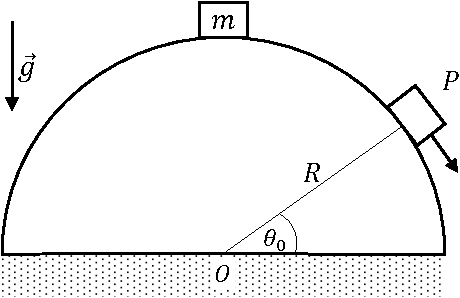
\includegraphics[scale=0.65]{2020-1/Imágenes/aux10/semiesfera_masa.pdf}
\end{figure}

% Para imágenes vectoriales -> el texto tiene que estar en LaTeX
% \begin{figure}[htbp]
%   \centering
%   \svgpath{../Imagenes/ejercicios}  -> .. irse pa'trás 
%   \includesvg{ej5.svg}
% \end{figure}

\end{enumerate}
\end{document}
